\documentclass[12pt,letterpaper]{article}
%\documentclass[14pt,letterpaper]{extarticle}

\includeonly{%
  abstract,
  introduction,
  methods,
  results,
  discussion,
  conclusions,
  appendix
}

% enable text super- and sub- scripts
\usepackage{xltxtra}
\usepackage{caption}
% let us typeset things inside the captions
\captionsetup{justification=justified}

\usepackage{graphicx}
% used for pmatrix
\usepackage{amsmath}
\usepackage{array}

% short space lists
\usepackage{enumitem}

% have a table that spans two pages...
\usepackage{longtable}

\usepackage[sc,osf]{mathpazo}
\usepackage[T1]{fontenc}
\usepackage{inconsolata}

% use fancy syntax highlighting provided by an interface to pygments
\usepackage{minted}

%\usepackage[margin=.75in,nohead,nofoot]{geometry}⋅
\usepackage[nohead]{geometry}
\usepackage{hyperref}
\usepackage[authoryear,round]{natbib}

% named colors, package already included with minted
\definecolor{DBlue}{rgb}{0.19,0.32,0.50}
\definecolor{DRed}{rgb}{0.7,0.22,0.21}
\definecolor{DGreen}{rgb}{0.15,0.41,0.15}
\definecolor{LGreen}{rgb}{0.01,0.62,0}

\newcommand{\R}{\textsf{R}}
\newcommand{\Rcmd}[1]{\texttt{#1}}

%\setlength{\parskip}{0.05in}
\linespread{1.2}

\geometry{
  body={6.5in, 8.75in},
  left=1.0in,
  top=1.0in,
  right=1.0in,
  bottom=1.0in
}

\hypersetup{
  colorlinks = true,
  urlcolor = black,
  citecolor = blue
}

\renewcommand{\theFancyVerbLine}{\sffamily\textcolor[rgb]{0.5,0.5,0.5}{\scriptsize\arabic{FancyVerbLine}}}

% fancy matrix environment which allows vertical bars
\makeatletter
\renewcommand*\env@matrix[1][*\c@MaxMatrixCols c]{%
  \hskip -\arraycolsep
  \let\@ifnextchar\new@ifnextchar
  \array{#1}}
\makeatother

\begin{document}
\title{\Huge{Assessing ship movements using volunteered geographic information}}
\author{Shaun Walbridge}
\maketitle{}

%\tableofcontents{
%\addcontentsline{toc}{chapter}{Table of contents}

%\begin{abstract}

ABSTRACTED

\end{abstract}


% from Oliver: WHY THE OCEANS ARE AWESOME, WHAT ADDRESSING SHIPPING DOES TO THE OCEANS, AND HOW KNOWING MORE WILL HELP SPECIFICALLY ADDRESS THESE ISSUES, with citations.

% - The importance of shipping means that data related to shipping is valuable
% - Leaves a gap in the data picture for scientific inquiry

% FRAME THE ISSUE BROADLY
% Shipping, the global ocean transportation of people and goods, provides a useful window into critical issues for geographic information science (GIScience), and its understanding has implications for a variety of applied fields including marine conservation, marine spatial planning, transportation geography, and navigation.  This work examines a synthesis of available shipping data.

The ocean is integral to supporting life, by producing much of the planet's biomass, acting as a critical step in the hydrologic cycle, and by regulating global climate. Oceans also support human needs by providing nutrition, resources, and an efficient medium for transportation. However, a confluence of changes is compromising the ocean's ability to support both marine life and meet human needs, with a recent study identifying climate change, fishing, and shipping as the greatest anthropogenic threats to marine health~\citep{Halpern2008}.  Shipping, the ocean transportation of people and goods, moves \$1.8 trillion dollars of trade annually, constitutes a \$300 billion dollar maritime industry, and plays a crucial role in the global transportation network, where it conveys 90 \% of world goods~\citep{oced2010,Rodrigue2009}. Preservation of the ocean's benefits calls for holistic management~\citep{Lubchenco2010}, which in turn requires detailed quantitative information. Current efforts have emphasized broad abiotic factors such as climate, and biotic factors such as fishing, but little work has examined the role of shipping, despite its importance to both the economy and the environment. This manuscript seeks to bridge this gap, by expanding our knowledge of shipping to address issues of marine conservation, marine spatial planning, transportation geography, and navigation.

%Shipping is also important in a broader context, and as we move toward the holistic management of the oceans, foundational data on human use is necessary~\citep{Lubchenco2010}. 

% EXPLAIN WHAT IS AND IS NOT KNOWN
% what we do know:
%\section{Existing Work}
Shipping produces many ecological impacts, but the effects largely remain out of sight, and little research looks beyond local scales. Ecological effects which have been examined include groundings, which cause direct effects like oil spills and habitat destruction, such as the \$3 billion Exxon-Valdez spill\footnote{The \$5 billion liability for the spill was so great that a now infamous financial instrument was manufactured to absorb it: the credit default swap.}.  Shipping contributes to climate change, where greenhouse gas emissions of the industry accounts for five percent of total man-made emissions~\citep{Eyring2009}, and its pollution causes 60,000 premature deaths per year~\citep{Corbett2007}.  Ship strikes also cause injury and death to marine mammals, and have driven whale population declines, for example the North Atlantic right whale (\textit{Eubalaena glacialis}), where human activity accounts for half of all fatalities, primarily caused by ship strikes and gear entanglement~\citep{Moore2007}. Globally, shipping has increased three-fold in the last 50 years, coinciding with increases in average vessel speed~\citep{Vanderlaan2009}. This combination has led led to large increases in shipping-induced marine mammal fatalities, despite efforts to track ship-whale interactions \citep{jensen2004large} and improvements to shipping lanes~\citep{Lagueux2011,Mckenna2012a}.

Ship ballast water, used to control vessel stability, also transports invasive species long distances, leading to widespread economic and biological losses~\citep{Ruiz2000,Rodrigue2009}. Transported species include plants, animals, bacteria, and human pathogens, resulting in major changes to many nearshore systems, particularly coastal lagoons and inlets~\citep{leppakoski2002baltic}.  Sound, which is efficiently transmitted by water, is used by manymarine species who have adapted sensitive hearing to forage and communicate. Engine noise from ships has led to extensive noise pollution, causing behavioral changes in a variety of marine species, and the loud sounds of naval activities can cause mortalities~\citep{Hatch2009}. With an improved understanding of shipping, further ecological and human impacts might also be identified.

% Other ecological and human impacts no doubt exist, but the poor understanding of shipping has left them unidentified~\citep{Davenport2006}.

% Oliver: Either I don't understand the however, or I don't understand what you mean by global phenomenon.  Were previous studies primarily local?  Are you going to integrate what previous studies have done?  Do you mean specific geographic areas, or specific areas within the limited field of shipping studies?
Little research has evaluated shipping as a global, interconnected system, where vessels move between a complex network of ports spanning the globe. The first work to examine the global shipping trade in an ecological context was \cite{Halpern2008}, a synthesis effort to collect information across habitat types and impacts. The work evaluates many human uses of the ocean, and gathers together global data to examine the cumulative ocean impact of humans, ranging from changes in sea surface temperature due to radiative forcing, to land-based nutrient runoff. The data used in this analysis to represent shipping, however, has limitations: It ignores vessel type, % TODO this is the first point at which I mention ship classes, what shipping *IS* should be explained earlier in the document.
 and contains information on only 12\% of the fleet. The ships it does include are also a spatially- and statistically-biased sample of the population \citep{Wang2007}, and the data vary between vessels, leaving many areas with known use missing from the model. Finally, the paper does not tackle modeling issues, but instead provides patterns without the context necessary to address deeper questions.

Another paper examining global shipping, \cite{Kaluza2010} instead focuses on the networks contained within shipping, providing an abstract network model of ship movement. Licensing data from Lloyd's Register Fairplay, % according to 'Data' section of Kalusa2010
 the authors aggregate port of call records, which are sequential lists of vessel location. They then extrapolate port-to-port links into routes, by combining land-based barriers with great circle distance calculations to select the path of a ship between two ports. This novel approach provides a measure of connectivity between port locations, and improves on the gravity model widely used to predict connectivity.  However, their work provides insufficient detail to extract true ship movement paths, a necessary step for effective spatial management. Instead, geographically referenced facts about movement are necessary. The data used also requires expensive licensing, making any extension of the work both financially prohibitive and limiting its accessibility. Despite largely ignoring geography, \cite{Kaluza2010} is currently the best examination of the global shipping trade.

% Much research focuses on specific areas within shipping, such as maritime awareness to detect anomalous behavior \citep{Tun2007}, tracking ship-whale interactions \citep{jensen2004large}, or shipping lanes to protect a species \citep{Lagueux2011,Mckenna2012a}.  Few papers tackle shipping as a global, interconnected phenomena, where vessels move between a complex network of ports spanning the globe. 

% ESTABLISH WHY THE QUESTION I HAVE IS AN IMPORTANT ONE

% due in part to the poor light penetration in water, limiting the effectiveness of remote sensing~

As we try to understand the health of the ocean \citep{Halpern2012}, we require quantitative data on the marine environment and its human use, both of which pose acute challenges to ocean scientists, due to our limited means to capture information in both the open ocean and at depth~\citep{Wright1997}. These data are necessary to inform decision-making, and are also important to minimizing the regulatory burden on the shipping industry. By managing shipping as a complex system, efficiency can be tied to improved environmental conditions. This work contributes foundational knowledge on the state and distribution of shipping, which can help understand this key user of the ocean, and identify key areas to examine for mitigating ecological impact.

%\section{Where this work comes in}

% SPELL OUT WHAT THIS STUDY DOES

% Halpern: This section jumps between many different topics and doesn't really explain them well enough to understand.  You either need to expand this a lot, or cut it way down and just state what the purpose of this study is.

% GIScience seeks to formalize our understanding of geographic information, and shipping can provide insight into areas of the GIScience agenda. 
% THIS IS GOING TO BE THE FIRST WORK TO *SHARE* DATA ON THE GLOBAL DISTRIBUTION OF SHIPPING, ALONG WITH DETAILED ATTRIBUTES NECESSARY TO DIG INTO THE TRICKY QUESTIONS WE HAVE IN ECOLOGICAL ISSUES.

% Attributes useful for ecological questions:
%    Noise: engine type, length, type
%    Ballast: type, length
%    Strikes: Maximum speed, type, draft

This is the first work to combine extensive global ship observations~\citep{VOSClim,Tetreault2002} with vessel identification records to both address questions on ecological effects of shipping, and to expand our understanding of the global shiping trade. Most previous works focused on regional problems, and the limited global work available used poor data~\citep{Corbett2007, Halpern2008}. Incorporating geographic quality checking methods~\citep{goodchildli2012} with volunteered geographic information (VGI, \citealp{goodchild2007citizens}), I provide a spatially resolved high resolution dataset which links individual ships with their movement patterns and vessel attributes. This dataset, when aggregated into multiple representations, allows us to answer open questions on topics including noise pollution, ship strikes, and invasive species introduction. 

% By fusing together data from multiple sources, here I build a dataset useful for interpreting the global shipping trade. While high resolution (spatially and temporally) volunteered information exists, its use has been limited to regional problems, and existing global work used poor data~\citep{Corbett2007, Halpern2008}. This paper contributes data predominantly within 100km of shores, where most human and biological users of the ocean persist, and building our knowledge of these areas is particularly valuable. Ship traffic is most dense, regulated, and complex within the exclusive economic zones of nations, and it is useful property that this data are dense within these areas.




% ... old stuff below

% Shipping places a growing demand on the ocean, transporting \$1.8 trillion dollars of goods annually, and providing a \$300 billion dollar maritime industry, representing one of the largest economic users of the ocean. This activity impacts both human health and the environment, such as the \$3 billion Exxon-Valdez spill\footnote{The \$5 billion liability for the spill was so great that a now infamous financial instrument was manufactured to absorb it: the credit default swap.}, but largely the effects of shipping remain out of sight. Documented effects include greenhouse gasses, accounting for five percent of total man-made emissions, and causing 60,000 premature deaths per year \citep{Corbett2007}. Ecologically, vessels cause ship strikes which can impair whale populations \citep{Fujiwara2001}, % XXX better refs? 
% transport invasive species, leading to widespread economic and biological losses, cause groundings with a host of direct effects like oil spills and habitat destruction, and produce noise pollution, leading to mortality events. Other ecological and human impacts are likely to exist, but remain unidentified, as shipping continues to be poorly understood~\citep{Davenport2006}. As we try to understand the health of the ocean \citep{Halpern2012}, we need detailed data, which poses an acute challenge to ocean scientists~\citep{Wright1997}. These data are necessary to inform decision-making, such as marine spatial planning, but is also important to minimizing the regulatory burden on the shipping industry: by managing shipping as a complex system, efficiency can be tied to improved environmental conditions.

% - Kaluza paper, based on Lloyd's data
%   + written for network theory audience
%   + data is port order for specific ships, which is used to come up with proposed routes of ships based on great circle distances (A to B to C)  
%   + problem - they don't actually know where ships travelled, which means results aren't helpful for problems where ship locations actually matter.
%   + can't share data, it's proprietary
%   + this paper is still the best that looks at shipping at a global level
%   + ignores geography

% - Work on global shipping
%   + Lots of papers that focus on specific parts of the shipping problem - few that take large perspective.
%   + Ben's Science paper
%    * first work that looked at global impact of shipping from ecological context, but wasn't focused on shipping
%    * first work to really look at how humans are affecting marine environment by synthesizing together all available global data
%    * problem with data is that it was based upon unrepresentative ships - missing whole categories of ships; only 12\% of fleet; representation issues (see Corbett \& Wang paper for details)
%    * second problem, uneven spatial distribution - tons of gaps. Data quality highly variable from ship to ship
%     - missing big areas of the ocean that we know lots of ships are using
%    * problem three - doesn't address data models (important for geographers); just says 'ships are here'.

% Moved this paragraph to CONCLUSION
% As noted by Goodchild, ``changing technology and economics are moving map production from a system of unified central production to a local patchwork, and the old radial system of dissemination is being replaced with a complex network''\citep{goodchild1999cartographic}. By using quality assurance methods from both computer science and geography, such as record linage and geographic validation, I can filter unreliable inputs. The near future will involve global, real-time, high resolution ship data \citep{JonesGoogle2012,carson2012satellite}, but I continue to need methods which accommodate data curation and integration, and allow us to address specific hypotheses. This is a key appeal of volunteered information: some problems of uncertainty become tractable with sufficient observation volume, as we can evaluate the distribution directly instead of relying on sampling methods.


\section{\textbf{Methods}}

% how did I solve the problem?

% FUNDAMENTALLY, doing synthesis on the shipping, with a set of simple rules to validate observations.
% shipping as sensor network -- a synthesis.

\subsection{Volunteered vessel information}

%"In short, changing technology and economics are moving map production from a system of unified central production to a local patchwork, and the old radial system of dissemination is being replaced with a complex network."
% -- Goodchild cartography paper, old and captures the change in production that is ongoing.

%\citep{elwood2011researching} includes refernce to these same layers, capturing data on 'core' data layers independently. Covers much of what Goodchild has discussed in terms of issues with VGI and its current 'cutting edge'
Historically, ship data was collected both by governments for internal use, and by private corporations with the intent to sell. As elsewhere in the production of geographic facts, a shift is underway which moves the emphasis away from top-down primary data collection, to instead relying on observations from a multitude \citep{goodchild1999cartographic,goodchild2007citizens,elwood2011researching}. Because of the limited authorative ocean information available, this has the potential to fundamentally change our use of the ocean.

% Using two kinds of volunteered ship data - needs to be handled in special ways:
% describe VOSclim data:
Ship captains have long taken climate observations alongside known location \cite{brohan2009marine}.  Building on this history, the Voluntary Observing Ship (VOS) \citep{VOSOverview} program has collected a dataset spanning over 20 years and covering 10\textendash20\% of commercial traffic within each year. The primary purpose of the data is to collect open-ocean climate observations, so many of the records lack ship attribute information, making trajectory reconstruction difficult. The data is contained within the greater International Comprehensive Ocean-Atmosphere Data Set (ICOADS) dataset, and though the data is both spatially and statistically biased \citep{Wang2007}, it still can serve as a useful 'training' dataset on ship movements in the open ocean. Here, we use VOS records from 2003--2011, a dataset of 92.4 
million records to provide validation and cross reference the rest of our observations. % XXX: this is really all of sailwx, not exclusively VOS.

% describe AIS data
The Automatic Identification System (AIS) \citep{no20041028,Tetreault2002} was developed to improve maritime safety and prevent collisions, by providing mariners local situational awareness. Locating the ships via global positioning satellite (GPS) signal, and broadcasting the location alongside other attributes (Table \ref{table:ais-broadcast-attributes}) regularly via VHF transceiver \citep{Itu-r2010}, mariners get a real-time display of local traffic, invaluable in inclement weather or rescue operations.  The International Maritime Organization (IMO) mandates that all ships $\geq\negthickspace 150$ gross tonnage (GT) or ships bearing paid passengers carry AIS units, which has lead to approximately 200,000 ships being outfitted with AIS equipment, including all tankers, cargo ships and passenger vessels. Because the intent of the system was to improve maritime safety, well-understood VHF radios were used, broadcasting to about 40km between ships. Since then, land-based users, including ports, maritime professionals and amateurs, have come to realize that by setting up VHF antennae, low-cost local ship traffic data can be obtained at a range of up to 100km. This has led to numerous sites providing real-time feeds of ship movement, such as MarineTraffic.com \citep{MarineTraffic}, aggregating the records from many land-based antennae (and more recently, satellite feeds) and displaying them over both web maps and via Google Earth. 

For this study, 15 months of AIS data were collected, from November 2011--December 2012, aggregating records from three online AIS providers: FleetMon, VesselTracker, and MarineTraffic. All three provide Keyhole Markup Language (KML, \citeauthor{KML}) files, intended to be used within Google Earth. Examining data availability (Figure \ref{fig:ais-coverage}) showed these providers had significantly different coverages. At ten minute intervals over the study window, I automatically downloaded these files from each of the providers. I then parsed the files to extract each observation within the dataset, wrote a library to normalize differences between the providers, and finally inserted the results into a spatial database, (PostGIS, \citeauthor{ramsey2005postgis}), an extension providing support for OGC simple features \cite{OGCSimple} on top of the PostgreSQL \citep{postgresql} object-relational database engine). Doing this over the study period produced 2.37 billion observations, which include ship location and time, but also additional attributes (Table \ref{table:ais-broadcast-attributes}).

Augmenting these datasets of ship observations, ancillary data was identified to provide validation against the raw observations. These include: 

\begin{enumerate}
  \item Vessel data, tabular lists of ships along with attributes, collected from both authoritative and crowd-sourced datasets.
  \item Port databases, containing coordinates and berth details for ports globally. Approximately 5,000 ports were identified from a variety of volunteered and authoritative sources.
  \item A high resolution land-sea mask, here derived from SRTM Water Body Data (SWBD), which classifies the world into either land or sea at three arc seconds resolution (~90 m) for the much of the world ($56\deg$ S to $60\deg$ N), a byproduct of the SRTM digital terrain project\cite{rabus2003shuttle}. Additional data was for the areas beyond these bounds.
  \item Approximate information on ship movement patterns, based on historical charts such as a CIA vessel movement chart from the cold war. (Figure \ref{fig:cia-shipping-map}).
  \item The original ship model I produced as part of the previous modeling effort \citep{Halpern2008}.
\end{enumerate}
% XXX EXPAND THIS LIST: ITU, FCC, Vesseltracker, DigitalSeas: THIS SHOULD BE MULTIPLE PAGES LONG...

\subsection{Validation}

The raw observations are full of caveats: because of the protocol design, there is no direct way of validating an incoming packet. So, as seen in (Figure \ref{fig:ais-obs-nov-2011}), many locations clearly on land have observations present, including a particularly thick band centered around the prime meridian. These records are more likely due corruption of longitude coordinate than reverence of Greenwich. Alongside transmission errors are operator error: the attributes which are sent alongside the time and position information are input by the mariners, and they may introduce errors in entry, or fail to update the attributes which change over time, such as the DESTINATION field. Each individual observation within this dataset is highly suspect, and generally the data is best treated as 'guilty until proven innocent'.

While there are numerous problems with the data, the large volume of data, and the compiled ancillary datasets, provide options to use the data via cross-correlation, improving accuracy and minimizing the number of raw observations required to build a model representation of the data. Two areas relevant to this problem are geographic data mining \citep{miller2009geographic}, and the recent work of \citep{goodchildli2012}. Here, we borrow the framework described in the latter work, and explore three avenues of quality assurance: crowd sourcing, social, and geographic approaches.

\subsubsection{Crowd-sourcing}
% based (large volume of obs, multiple sources. Crowdsourced ref material)
% XXX EXPAND EXPAND, talk about authority and what it means
While \citep{goodchildli2012} found that crowd-sourcing was generally inadequate for VGI, it can function when the domain is limited and the pool of expertise is vast (as in the case with much open source software). In one sense, crowd-sourcing comes into play in this data when multiple radio towers of differing quality and origin receive records, across a variety of sources. Cross-referencing these sources then provides a consistency, though this doesn't rely on many citizens cross-referencing, but rather validates across their equipment.

\subsubsection{Social}
% XXX EXPAND LIKE A MOFO
Mariners do provide regular updates to the various online services as to their attributes, so the attribute data pulled from these sources tends to be high. The ship operators often have the best working knowledge ships' data, much like someone who lives in a specific neighborhood is likely to have a better understanding of local geography. The ship operators can then communicate the data up to various shipping related aggregation sites, who operate the higher levels of the hierarchy, and rely on a group of trusted users for vetting incoming updates.

\subsubsection{Geographic}
% XXX this is BLEH right now, make it not crap.
This brings us to perhaps the most important validation technique: using geography to validate the records. In this case, the individual observations are time-stamped points which precludes complex rule-based geometry checks, but we can rely on a few simple sets of tests:

In addition to our point location $\langle x,t \rangle$, we have multiple attributes $\langle z \rangle$ attributes alongside it, proving us a spatio-temporal observation $\langle x,t,z \rangle$. By cross-referencing the attributes, we can get a sense of how likely the attribute-only component of the record is, and infer from that how likely we are to have a valid geometry and timestamp.

We can also impose some basic validation on the geometries by referencing other geographic facts, as is used in the most pedestrian of GIS functions, the overlay analysis. By checking the data against a land-sea mask, we can make estimations as to when the provided location is a physical impossibility. One trick to this is that many ships do travel by river, so these rules must be careful to define what is a traversable area. Additionally, shallow water bodies impose additional constraints on many ships with positive draft. This could be validated (showing for example, the large berth oil tankers keep from land), but hasn't been implemented here.

For many classes of vessels, ships move between ports. Ships which exhibit movement patterns inconsistent with this goal are suspect, though there are other 'nodes' in the ocean which require inclusion, such as ballast water exchange points, such as the one located 200km offshore of California (Figure \ref{fig:cal-cargo}), and canals, which provide a means of ships to move between otherwise inaccessible locations. However, this remains a powerful validation technique: because the high resolution data is clustered around the shores with strong coverage at the ports, we get a disproportionately good look at the vessels in transit between this constrained set of locations.

As in many large dataset, the distribution of observations per ship follows an approximate power-law distribution. Using the raw number of observations received in our 15 month window provides another filter. A peak in the kernel density estimation (Figure \ref{fig:obs-per-vessel-log}) is seen around $10^4$ observations, with a clear drop-off after $10^5$ which is consistent with the theoretical maximum (one observation in every sample) of about $6.8 \times 10^5$.

\begin{figure}[htbp]
  \centering
  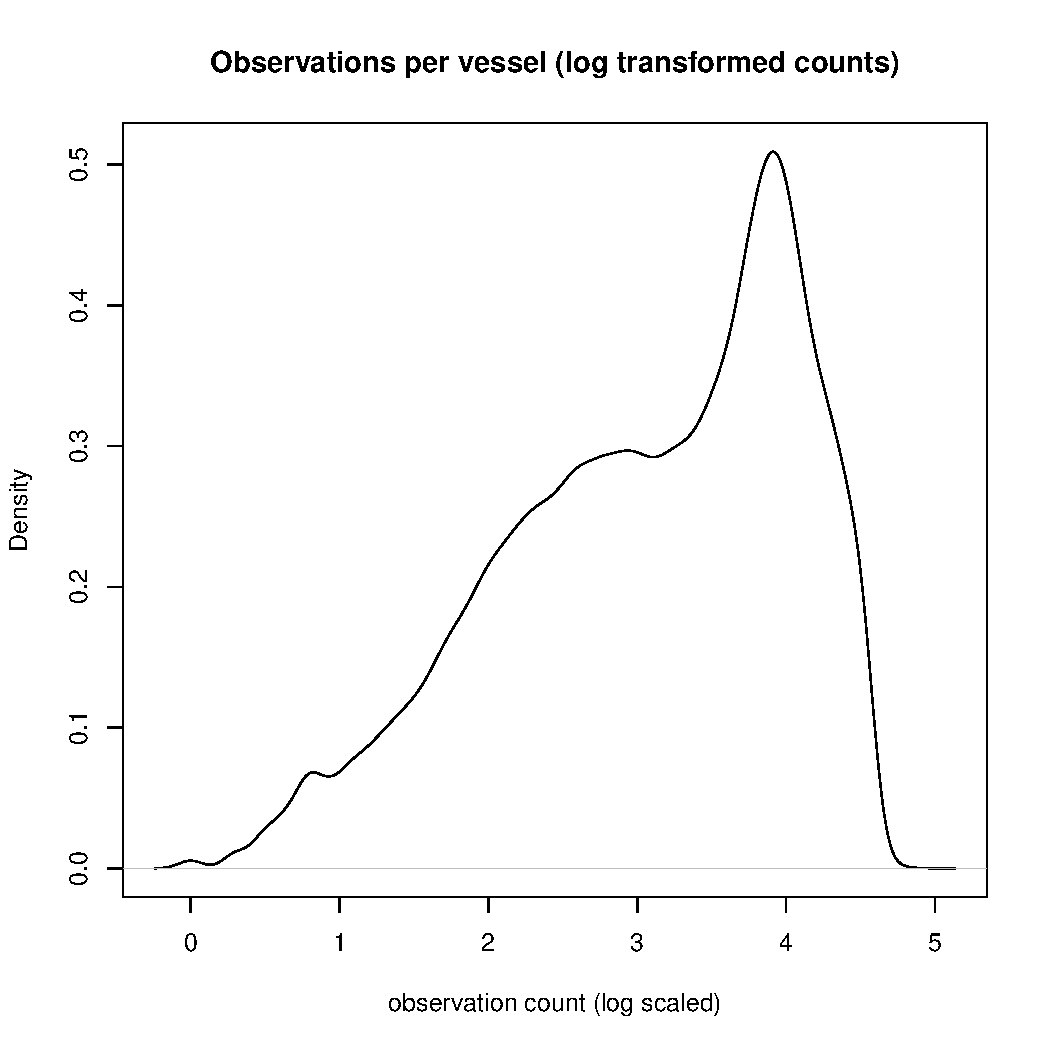
\includegraphics[width=100mm]{figures/obs-per-vessel-log.pdf}
  \caption{Number of observations per vessel, log scaled.}
  \label{fig:obs-per-vessel-log}
\end{figure}


% highlight importance of geometry + ATTRIBUTES. one alone is insufficient, both can be powerful.

% - geographic filtering 
%   + PORTS
%   + LAND/SEA MASK
%   + ...
% Link above with Goodchild thoughts on VGI and quality.

%An aside on 'ships' - ships can have multiple callsigns, MMSI idenfiers, and other data which ideally would locate a specific vessel. We handle this ambiguity methods -- a full version of this can go into supplementals, but worth covering here, because we can map \textbf{type} from observed behavior -- fishing vs. cargo vs. cruise is all obvious when looking at the movement patterns (fold into above 'filtering process' section)

Another important point is that while ship attributes provide us some details as to their nature, categories (such as tanker or cargo) are not based purely on attributes, but also include movement patterns. This is a distinguishing characteristic between the data, as different classes of vessel show distinct movement patterns, which is useful both in validation, and as an output product, since vessel classes have differing effects and interactions. Because this data is stored in a spatial database, we can link any derived representation back to the records that formed it. While this is a common feature of spatial databases, its an important trait since generally scientists are provided a simple 'end product' without the provenance trail which backs the specific data being provided.

% XXX above is good, expand it

%Can link data representations all the way back to attributes of raw data [note: this is true in many spatial databases, right? what makes it special here?]
% - often a requirement but only get 'end products' instead without detailed attributes, or conversely all details on one ship but no way to move between realms fluidly.

% overview of summary statistics of data
\begin{table}[htbp]
  \begin{tabular}{rrrrrr} %{\centering\arraybackslash}p{2cm}>{\centering\arraybackslash}p{5cm}>{\centering\arraybackslash}p{9cm}}
    \hline
    Type & Vessels \textit{(AIS)} & Vessels \textit{(VOS)} & fleet size & coverage (\%) & observations (M) \\

    \hline
    Cargo & 25214 & 5838 & 33392\textsuperscript{1} & 75.6 & 665.45 \\
    Tanker & 9758 & 2375 & 14068\textsuperscript{1} & 69.4 & 264.42 \\
    Passenger & 4007 & 777 & 6370\textsuperscript{1} & 62.9 & 142.16 \\
    Support & 9954 & 735 & 25234\textsuperscript{1} & 39.4 & 298.02 \\
    High-speed & 404 & 81 & 1178 & 34.3 & 2.52 \\
    Fishing & 11186 & 349 & 51200\textsuperscript{3} & 21.8 & 6.87 \\
    Pleasure & 20727 & 661 & 800,000\textsuperscript{2} & 2.59 & 267.48 \\
    Other & 9507 & 1400 & -- & -- & 4.75 \\
    Authority & 656 & 55 & -- & -- & 1.44 \\
  \end{tabular}
  \caption{Summary of analyzed ship data\\
  1. \cite{Equasis2011}.\\
  2. \cite{westwood2001global}.\\
  3. \cite{FAOfishing}.}
  \label{table:ships-by-type}
\end{table}
% XXX: high-speed craft from ISL? can't find original ref
% NOTE: the FAO estimates the _full_ fishing fleet size at 4 million vessels, the size clearly has an important effect.
% select validation_class, count(validation_class) FROM sailwx.obs_lines o LEFT JOIN clean.ships s ON s.id = o.ship_id WHERE validation_class is not null GROUP BY validation_class;

% tanker           |  2375
% high-speed       |    81
% cargo            |  5838
% passenger        |   777
% support          |   735
% authority        |    55
% fishing          |   349
% pleasure         |   661
% other            |  1400

% SELECT validation_class, COUNT(validation_class) FROM clean.ships WHERE validation_score > 0 GROUP BY validation_class;
% tanker           |  9758
% pleasure         | 20727
% fishing          | 11186
% high-speed       |   404
% cargo            | 25214
% passenger        |  4007
% other            |  9507
% support          |  9954
% authority        |   656

% classes from joined clean.ships table [RAW, both good and 'bad' records.]
% 'high-speed': 1178
% 'passenger': 7182
% 'cargo': 32970
% 'support': 21425
% 'authority': 1308
% 'fishing': 28544
% 'pleasure': 57617
% 'tanker': 20503
% 'other': 29077


% Equasis 'state of the fleet' report (2011):
% NOTE: also has a helpful list in annex I of what comprises each class.
%   container/cargo [total: 
%     general cargo: 17034
%     specialized cargo:  250
%     roro cargo: 1537
%     container ships: 4974
%     bulk carriers: 9597
%   tankers:
%     oil and chemical tankers: 11828
%     gas tankers: 1574
%     other tankers: 666
%   passenger ships: 6370
%   offshore vessels: 6692
%   service ships: 4442
%   tugs: 14110

% as listed in maritime economics 3e (2007): (all over 10,000 dwt only):
% http://books.google.com/books?id=PAi04qzmfucC&pg=PA69&dq=shipping+cargo+fleet&hl=en&sa=X&ei=Ei2YUOTaNs3oiwKhy4D4CA&ved=0CDYQ6AEwAA#v=onepage&q&f=false
% tankers: 8040
% bulk carriers: 14756
% general cargo: 25784
% specialized cargo: 6978
% total cargo: 47433
%   tugs: 11097
%   dredgers: 1612
%   cruise: 452
%   ferries: 3656
% total non-cargo: 26880
% total fleet size: 74398

\subsection{Data Representations}

% It is necessary to have multiple representations of the data - the data model must flow from the question asked (goodchild, also anything in ebook on GISci?)

After filtering and validating the data as described above, we want to begin building data representations which allow us to answer some of the questions highlighted in the introduction. As is the case in many datasets, there is no single optimal representation, but instead a set of representations which, when matched to particular uses, allows us to address interesting questions.

Here, we look at how maintaining both discrete object and continuous fields representations (Figure \ref{fig:representation-in-gis}) allow us to addressed questions about shipping, including its ecological effects. The point data alone is insufficient for making predictions related to these phenomena, but neither can we incorporate too much complexity or we risk making computation infeasible and the data requirements beyond what we can collect \citep{de2007geospatial}.

% Some of the effects. link up how specific effects could be monitored by our different repsentations. Can't just use points to predict phenomena of this nature, but can't incorporate full complexity of reality either; chosen representations are a compromise between those two extremes.

% As in \ref{fig:representation-in-gis}, we can keep track of the ships in a discrete object representation, and after filtering the observations, converting the individual ship locations into movement tracks.

% Merger of data - which can give a single representation of the data

\begin{figure}[htbp]
  \centering
  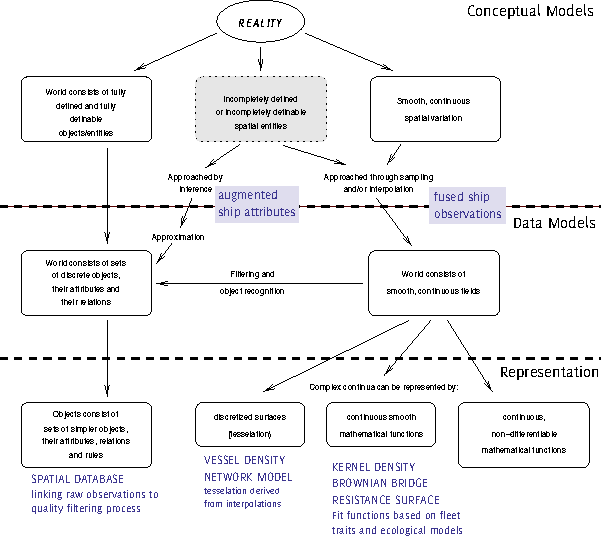
\includegraphics[width=160mm]{figures/representation-in-gis.pdf}
  \caption{GIS abstractions, this work's specific {\color{DBlue} additions in blue}. Adopted from \cite{Bivand2011}}
  \label{fig:representation-in-gis}
\end{figure}

% It is necessary to have multiple representations of the data - the data model must flow from the question asked (goodchild, also anything in ebook on GISci?)

%Want to link representation to USE, lack of a single simple view which meets all needs. counterpoint to the 'single metric' perspective. 
% [have note: 'link to stats', but now unsure what that means].

% Store the raw observations in a spatial database (PostGIS), use parallelized code to quickly aggregate the results.

\subsubsection{Raw point data}
 \begin{itemize}
   \item geoatom with time $\langle x,t,z \rangle$
   \item formalize what these observations mean
   \item apply filtering using space-time + attributes
 \end{itemize}

We have records sampled at 10 minute intervals (600 seconds). This is a reasonable approximation of paths for most of the observed movement patterns, and doesn't differ significantly from others who have aggregated to remove for noise (\cite{Vries2009}, which uses piecewise aggregate approximation with w = 30 (300 seconds) to 'strike a good balance between capturing the general movement and ignoring noise'. % NOTE: this is a filtering technique, so it isn't a direct mapping onto the reduced fidelity data we're using.

Spatial databases historical focus on accuracy \citep{goodchild1989accuracy}

\subsubsection{Tracks}
 \begin{itemize}
   \item link to time geography... Hagerstrands conceptual framework... Literature on T-GIS as tracking.
   \item Goodchild lecture on T-GIS mentioned track interpolation, inferences about activity, track convergence, etc

 \end{itemize}
 % [perhaps drop this for the time being... don't have lit built up on it, unless we can use the anomaly detection stuff]

\subsubsection{Field-based models}

Used kernel smoothing to produce these field-based estimates.

\paragraph{Density estimates of ships by type}

Why this matters: the view most people want to see; counts of X where and when. Useful for MSP, conflict resolution, detecting conflict zones, etc

\paragraph{Speed density estimations of ships by ship type}

Speed plays a critical role in determining the survivability of marine mammals from collisions (Vanderlaan, others), and speed also is the primary knob on the emissions profile of a particular vessel.

CLARIFY: what are the other effects of speed? anomaly detection?

\subsubsection{Network model of ship travel}

Some analyses require 'factoring out' geography to the extent possible, such as ecological models (Tilman book), Economic, et cetera. Network theory provides a useful basis of analysing geographically explicit data in a mathematical framework which can incorporate some of the geographic constraints while eliding many details necessary in a spatially-explicit model.

Best thing here is Kaluza but they totally lost the geography in transit -- can produce a middle ground model which has geographic nodes and edges, but still retains the rigour of the network model. Can get both!

% Paragraph from one of my position papers --
% One model I’m particularly interested in is hybridized network models using tools like NetworkX, which have the attractive property of allowing mixed field/object representations of the same data simultaneously, hence escaping the common limits of networks as mentioned in ? of every link or edge requiring a discrete value. By imbuing a network model with object-oriented features, some of the challenges I’ve been having representing my ship traffic data vanish. An- other advantage of manipulating graphs as a primitive is their widespread support, including general purpose graph databases which are particularly taking off in the semantic space.

% another pp from a position
% This becomes particular important as the tools of spatial thinking extend across disciplinary boundaries, both in the social and physical sciences (Goodchild and Janelle, 2010; Tilman and Kareiva, 1997). Other domains, such as ecology and economics, are coming to terms with the fact that their historical approaches to keeping simple models (and by extension, limiting model scope to their domain) ignores important spatial context which naturally arises at the unit of analysis (Tilman and Kareiva, 1997; Krugman, 1991).



% -----------------------------------------------------------------------------


% One advantage of linked data or hierarchical models is allowing cross-correlation among many datasets which may improve accuracy with less new measurement required. This is one appeal of volunteered geographic information: some uncertainty problems become tractable when we have orders of magnitude more observations , as we can evaluate the probabilistic distribution of a phenomena not by specifying a priori distributions, but instead allowing the large volume of samples to provide a distribution. Efforts to accomplish this include geographic data mining Miller and Han (2009).


% Volunteered Geographic Information (VGI) Goodchild (2007), involves participation of citizens in the production of georeferenced facts. Extending the ideas of User-generated content (UGC) to the specific nature of geographic information, a transition away from authority-based production means that information provided is often asserted rather than filtered through a formal quality control process. This shift requires new approaches to validate and quality-control VGI, while retaining its benefits in turnaround time and production cost. In Goodchild and Glennon (2010), a case study of disaster response is taken up, where real-time information is critical to save lives and minimize property damage, and the appeal of VGI is obvious.  

%\ldots

% Following up on Goodchild and Li (2012), three mechanisms for quality assurance are men- tioned: crowd-sourcing, social groups, and geographic. Hybridized approaches which use all three would be useful: rely on the size of the participation base to cross check (and improve sample size from a statistical perspective), use a social structure to defer in disputes and confer some of the virtues of authority, and use filtering which takes into account abstract geographic rules to impose constraints on the data.

% The approaches of machine learning and geographic data mining again seem particularly relevant here: as we build up cross referenced datasets on participants, we can infer much more despite the limits of each individual observation. In effect, this is what Currier et al. (2012) suggests, by adding information on who volunteers what, we can move toward solving the lingering semantic issues present in ’universal’ geographic information. One risk: much of the correlated information is controlled by a handful of organizations such as Google, Facebook and Twitter, which sell that information back to advertisers Lanier (2010) which limits the possibility of truly connected geographic facts, as the organizations have incentives to keep large parts of their information private.

\subsection{Record Linkage}

% XXX open problem: what designates a 'ship'?
%   Hal: `The biggest flaw is that, long ago, I assumed one ship == one callsign. It turns out, of course, that a single ship can have multiple callsigns (due to sale or reflagging), and that a single callsign can be assigned to multiple ships (e.g. NOAA, and also the Queen Mary/Queen Mary II). So the db really needs its own internal ship UID.`

%  Hal, on 'using MMSI + IMO + Callsign'--  Yeah, that still misses reflagging. I think what I will end up with is a "find-or-create ship with IMO,MMSI,Callsign", together with a manual process for me to force the database to combine two different ship UUID's that actually refer to the same ship. Even that isn't enough, because we see misprogrammed AIS units with dummy MMSI's, and fleetwide MMSI's."

%    ... Almost want a probabilistic model of what ship it is based on the information we do have reliably, and cross-validation with the various online databases... perhaps even validation with Equasis? Could do this for a small subset of the ships, but clearly not them all.

% XXX   - create a ship 'UUID' like feature which incorporates the different aspects: IMO, MMSI, Callsign, Name... we care about specific _ships_ not necessarily what line they're running under or other changes, though this is useful information for certain classes of questions.

%  - collapse all redundant columns from the database once we have this hybrid observation model and can safely assign individual records to a particular ship (instead of a guess based on say, MMSI, which may be misprogrammed).

% XXX mention the ontology work in this space: there are people thinking about this stuff, but it isn't where we need it to be.
% \cite{Vries2009}
% IALA Guideline No. 1028 On The Au tomatic Identification System (AIS)

By combining authoratative data from a variety of sources (Table \ref{table:ships-data-sources}), we can reconcile our observations with known ship records, and greatly improve the quality of the resulting ship movement models. Though authoratative, the sources are also inconsistent, and require an initial step of cross-linking records, an approach commonly used in medical records [cite] and computer science [cite].

% table describing sources
% SOURCES: ship-id-model.txt
%          ship-id-model/linkages.txt
\begin{table}[htbp]
  \begin{tabular}{rrrrl}%{\centering\arraybackslash}p{2cm}>{\centering\arraybackslash}p{5cm}>{\centering\arraybackslash}p{9cm}}
    \hline
    Source & Code & Records & Cross-linked & Attributes \\
    \hline
     Digital Seas & DS & 212166 & 68002 & {\footnotesize name, IMO, MMSI, callsign, type, width, length} \\
      FCC\textsuperscript{1} ULS\textsuperscript{2} & FCC & 319964 & 24531 & {\footnotesize name, MMSI, callsign, class, gross gonnage, length} \\
      ITU\textsuperscript{3} MARS\textsuperscript{4} & ITU & 372183 & 75928 & {\footnotesize name, IMO, MMSI, callsign, class, owner, gross tonnage}\\ 
     VesselTracker & VT & 126534 & 83372 & {\footnotesize name, IMO, MMSI, callsign, class, length}
  \end{tabular}
  \caption{Ship data sources.\\ 
  1. Federal Communications Commission \\ 
  2. Universal Licensing System \\
  3. International Telecommunication Union \\ 
  4. Maritime mobile Access and Retrieval System}
  \label{table:ships-data-sources}
\end{table}

%     International Telecommunication Union: Maritime mobile Access and Retrieval System (MARS) & ITU & 372183 & 75928 & name, callsign, mmsi, class, owner, imo, gross tonnage\\ 
Here, we build a probabilistic model which evaluated all possible pairwise combinations between all source records. By using the methodology of record linkage \cite{Christen2012}, we built a set of rules to map records between the six possible source pairs. Each pair was evaluated for attributes which had consistent data, and matched against these columns. The software package used, (FRIL, \cite{Jurczyk2008fril}), provides an Expectation Maximization algorithm to iteratively optimize the weighting of columns, but due to the volume of data in our sources, this proved inefficient. Instead, samples of the data were examined, and the criteria were set by manual tuning both the weightings and acceptance levels to match a training dataset of valid linkages (Table \ref{table:ships-record-linkage-methods}). % XXX HUURR, write this better

For most fields, either the 'equal fields' (both fields are exactly the same) or the Jaro-Winkler distance metric were used. Jaro-Winkler has a useful properties for this data: it is effective on both numeric and textual data, and is particuarly useful in picking up the kinds of errors inherent in user-entered and sometimes poorly validated data sources such as those used in this study. A study of a variety of string comparison metrics \cite{Cohen2003} found it % XXX what?

CATCHING ERRORS:
 detecting errors in this data is particularly problematic because the records are highly correlated by nature -- similar imo, callsign and name for two different ships in the same fleet. have to keep those separate while linking small diferences due to entry error.

 wrote validate-ds-vt.py which encapsulates a bunch of useful rules for the edge cases, and I've visually inspected the results. it does a good job of finding our other 'missing matches'.

% TODO: perform data validation on these observations with Equasis. Sample a handful of records from each class, then perform the validation.
While some of our input linkage datasets are semi-authoratative, the best data remains commerical. As another validation step, a 1\% sample of the records were compared to those provided in Equasis \cite{Equasis2011}, which includes validated records from the commerical fleet. (VALIDATION STILL IN PROGRESS).


% table describing the record linkage technique used for each data source
% SOURCE: record-linkage/FRIL/config/*.xml
\begin{table}[htbp]
  \begin{tabular}{rrrrrr} %{\centering\arraybackslash}p{2cm}>{\centering\arraybackslash}p{5cm}>{\centering\arraybackslash}p{9cm}}
    \hline
    Source $A$ & Source $B$ & acceptance level & column & distance metric & weight \\
    \hline
     DS & ITU & 92 & callsign & Jaro-Winkler\textsuperscript{1} & 50 \\
        &     &    & MMSI & equal & 40 \\
        &     &    & name & Jaro-Winkler & 40 \\
     DS &  VT & 85 & callsign & Jaro-Winkler & 60 \\
        &     &    & IMO & Jaro-Winkler & 20 \\
        &     &    & name & Jaro-Winkler & 20 \\
    FCC & ITU & 85 & callsign & Jaro-Winkler & 95 \\
        &     &    & name & Jaro-Winkler & 5 \\
    FCC &  VT & 95 & callsign & Jaro-Winkler & 66 \\
        &     &    & name & Jaro-Winkler & 5 \\
        &     &    & MMSI & Jaro-Winkler & 24 \\
        &     &    & length & equal & 5 \\
     VT & ITU & 80 & callsign & Jaro-Winkler & 20 \\
        &     &    & MMSI & Edit Distance & 30 \\
        &     &    & name & Jaro-Winkler & 10 \\
        &     &    & IMO & Jaro-Winkler & 40 \\
     DS & FCC & 95 & callsign & equal & 99 \\
        &     &    & name & Jaro-Winkler& 1 \\
  \end{tabular}
  \caption{Ship record linkage methods used. \\
    \textsuperscript{1} Jaro-Winkler distance \cite{winkler1990string}: length $l = 4$ and scaling factor $p = 0.1$}
  \label{table:ships-record-linkage-methods}
\end{table}

After pairwise linkage, matched records (Table \ref{table:ships-record-linkage-results-summary}) were further cross-referenced, % XXX HOW? create-ships-table.py contains the logic.
 to account for the fact that the same ship often appears in many of our sources. The number of links per ship averaged 3.5 ($\mu = 3.49, \sigma = 0.828$) % XXX STATISTICALLY SIGNIFICANT? the vast majority only have 3-4 links. Tried fitting this data to a variety of distributions, it can be done, but for what end? the 'high' values really indicate errors, and these should be separated out to their relevant subships.

% THEN WHAT...


% XXX what follows is the math for the Jaro Winkler equations, worth mentioning as they describe the primary method used for linking our records together.
The Jaro-Winkler equations (described in Appendix \ref{sec:record-linkage-appendix}) provide ...


\subsection{Geographic Validation}


A high resolution land-sea mask, here derived from SRTM Water Body Data (SWBD), which classifies the world into either land or sea at three arc seconds resolution $56\deg$ S to $60\deg$ N, a byproduct of the SRTM digital terrain project. Additional data was for the areas beyond these bounds.


% A concise report of your results. A final report is not a lab log book, so you do not need to include details of every calculation or include every graph.  Most readers get bored if there are too many very similar graphs in a paper. The key requirement is to report all findings that relate directly to your goals and that will be referred to in the discussion.  

% Avoid having the text in the Results section be a simple list of each result or statistical test – integrate, summarize, synthesize, and point out the most important messages you want your readers to take away from the paper.

% What really matters from what we've done?

\section{Record Linkage}

Record linkage matched 30-50\% of each record source pair (Table \ref{table:ships-record-linkage-results-summary}), and additional validation boosted this even further. That authoritative data is inconsistent points toward needing better unified and public identifiers than are currently exist.

After pairwise linkage, matched records were further cross-linked, % XXX HOW? create-ships-table.py contains the logic.
 to account for vessels appearing in multiple sources. The number of links per ship averaged 3.5 ($\mu = 3.49, \sigma = 0.828$), % XXX STATISTICALLY SIGNIFICANT? the vast majority only have 3-4 links. Tried fitting this data to a variety of distributions, it can be done, but for what end? the 'high' values really indicate errors, and these should be separated out to their relevant subships.
though this distribution is skewed by a handful of vessels which were linked to many vessels incorrectly. 
% XXX move this table to an appendix? doesn't really help tell the story.
% table describing # of records linked betwen each source
% SOURCE: ship-id-model/matches.ods
\begin{table}[htbp]
  \begin{tabular}{rrll} %{\centering\arraybackslash}p{2cm}>{\centering\arraybackslash}p{5cm}>{\centering\arraybackslash}p{9cm}}
    \hline
    Source $A$ & Source $B$ & matched records & \% possible matched \\
    \hline
     DS & FCC &  3481 & 50.35\textsuperscript{1} \\
     DS & ITU & 41380 & 30.73 \\
     DS &  VT & 72286 & 53.68 \\
    FCC & ITU & 27874 & 50.58\textsuperscript{1} \\
    FCC &  VT &  5282 & 53.23\textsuperscript{1} \\
     VT & ITU & 54727 & 43.25 \\
  \end{tabular}
  \caption{Ship record linkage results summary. \\
    1. FCC data is US only, \% possible is of US-only data from these sources.}
  \label{table:ships-record-linkage-results-summary}
\end{table}

\section{Geographic Validation}

The land-sea mask developed (Section \ref{sec:land-sea-mask}) was compared against each observation: is the point contained within a water body? However, this simple validation technique was insufficient to resolve many observations, which lie at the edge of the two classes when docked % XXX Oliver Do docked ships really belong in a shipping dataset anyway?
 and moving near shore % XXX Oliver How near shore?  Are there that many boats that actually travel in this zone?  I imagine Costa Concordia.
(Figure \ref{fig:longbeach-validation}). Due to this and other limitations, the observations 'on land' were retained for the rest of the analysis, but perhaps a better approach would be to apply a local density estimation on the vessels, and determine a mask based on thresholding the data. Instead, most of the on land observations were filtered by using our track generation rules, which by restricting vessel movements to a possible range, generally remove individual erroneous observations, but a more robust technique would be useful for systematic errors.

% XXX: how did we improve data quality by using geographic filtering? what does that tell us, and why does it matter?

\section{Ship results}

\subsection{Speed}
\begin{figure}[htbp]
  \centering
  \includegraphics[width=150mm]{figures/speed-boxplot.pdf}
  \caption{Boxplot of validated ship speeds.}
  \label{fig:vessel-speed-boxplot} % XXX Oliver: and? in theory I shouldn't have to read that part of the paper.
\end{figure}

Ship speed is an important predictor for a variety of questions, but is challenging to represent spatially, as it is sensitive to the observation frequency in a particular location, along with accurate distance and time measurements. To get a general sense of ship speed, the speed distribution of each vessel class was examined, both through simple boxplots (Figure \ref{fig:vessel-speed-boxplot}), and through a more nuanced kernel density estimation (Figure \ref{fig:vessel-speed-density}). The density estimation shows that for many classes, distinct speed patterns are clearly visible. For example, support vessels, which include tugs and barges move much more slowly than high-speed transport vessels. Other classes are less distinct in speed signature: cargo and tanker vessels have surprisingly similar average speeds, though by breaking this down spatially (Figure \ref{fig:speed-ship-map}), we can see a more nuanced story.

% graphs of SHIP SPEED by type, either using kernel estimation or simple histograms depending on the clarity of the data.
\begin{figure}[htbp]
  \centering
  \includegraphics[width=150mm]{figures/speed-comparison-qqplot.pdf}
  \caption{Distribution of validated ship movement speeds, computed using kernel density comparisons, as described in \citep{bowman1997applied}.}
  \label{fig:vessel-speed-density} % XXX FIX LABELS, ADD UNITS, WHAT DOES THIS MEAN?
\end{figure}

\begin{figure}[htbp]
  \centerline{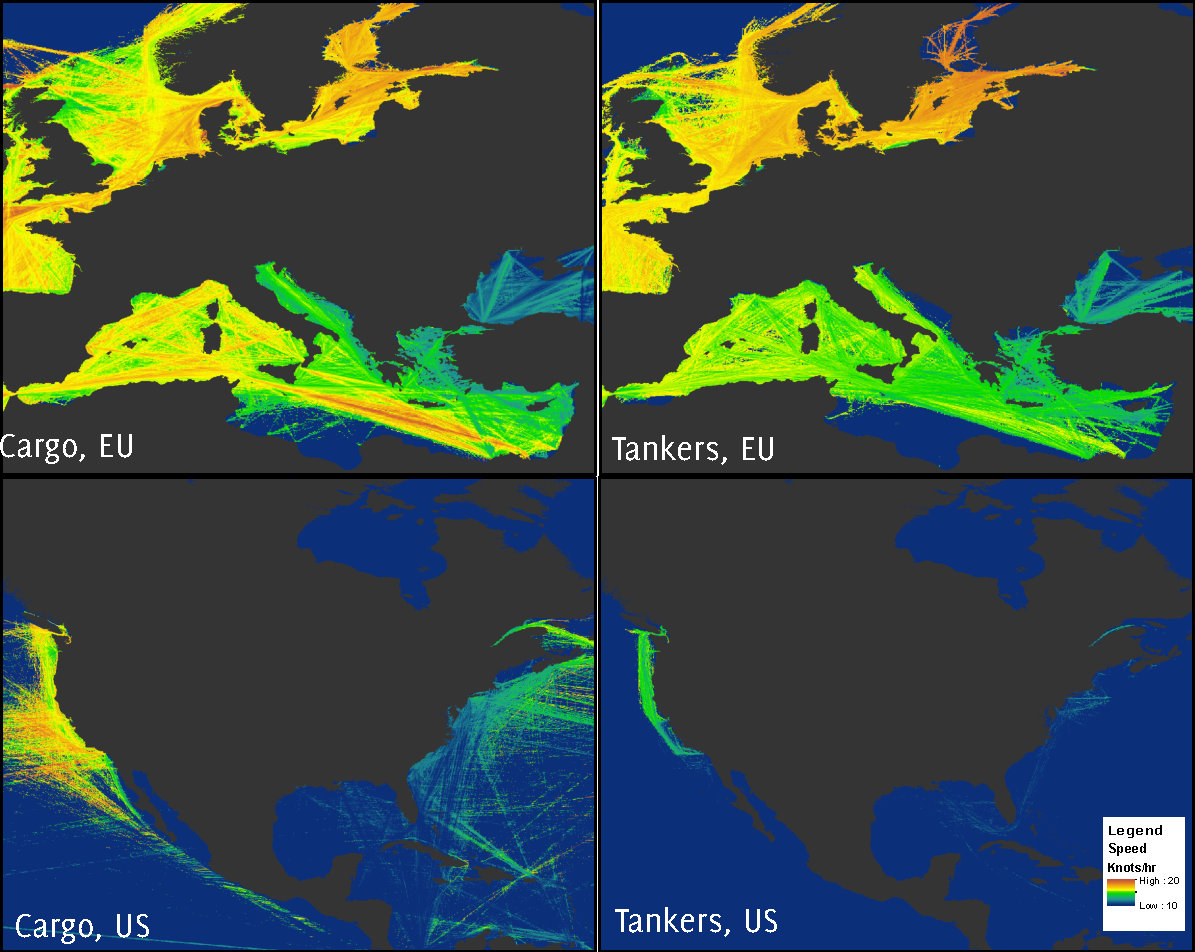
\includegraphics[width=160mm]{images/speed_map_labeled.pdf}}
  \caption{Average ship speed examples. Scale shows 10-20 Kts/hr range for all vessels. Of note is the large difference in speeds between the opposite shores of North America.}
  \label{fig:speed-ship-map}
\end{figure}

\subsection{Density}

The density maps show the dramatically different movement structure of the major vessel classes: cargo, tankers and passenger ships all exhibit important differences in their movement. 

\begin{figure}[htbp]
  \centerline{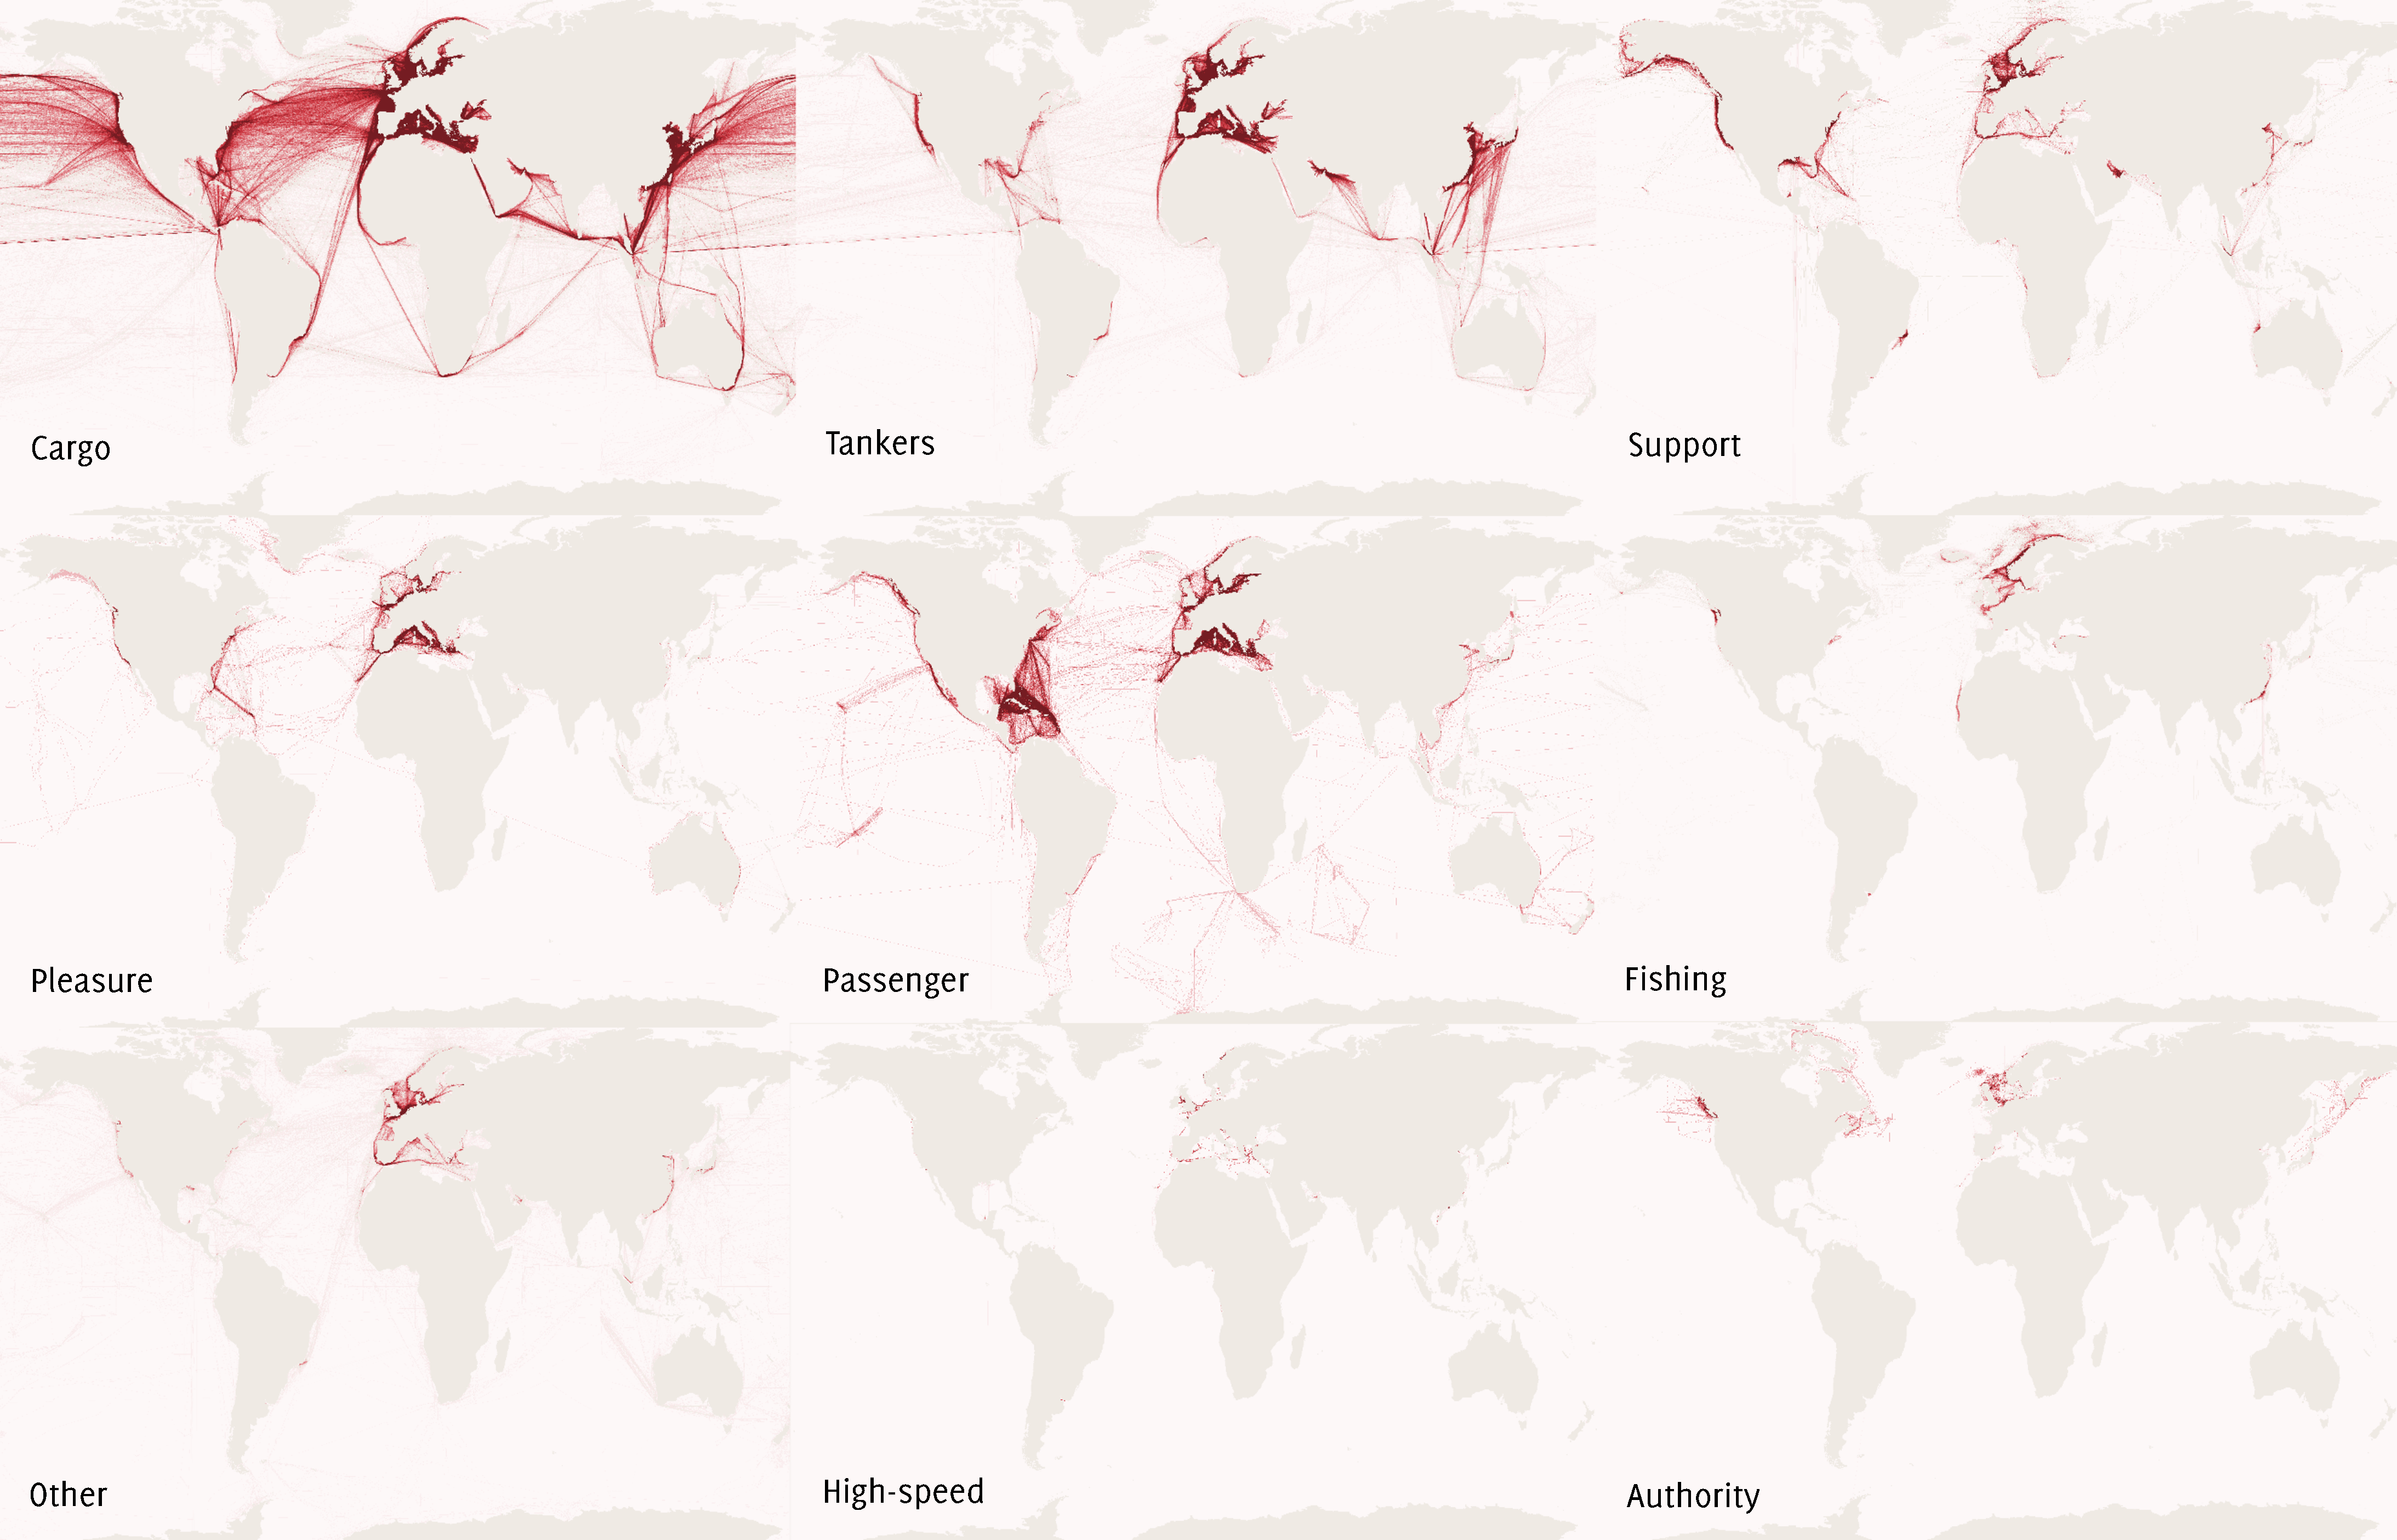
\includegraphics[width=160mm]{figures/9fold-map-labeled-resized.pdf}}
  \caption{Ship movement densities. first row: cargo, tankers, support. second row:  pleasure, passenger, fishing. third row: other, high-speed, authority.}
  \label{fig:9fold-ship-maps}
\end{figure}


\subsection{Spatial Autocorrelation}

% XXX Oliver Oh.  I thought you had a regression somewhere, in which case Moran's I tells you something about whether spatial autocorrelation is weakening your inference.  In this case, I'd have gone with a variogram.
Geographic features tend to be clustered, exhibiting spatial autocorrelation. Here, we use Moran's I to compute global autocorrelation statistics for our density rasters:
\begin{equation}
I = \frac{n}{\sum_{i=1}^{n}\sum_{j=1}^{n}w_{ij}}
\frac{\sum_{i=1}^{n}\sum_{j=1}^{n}w_{ij}(x_i-\bar{x})(x_j-\bar{x})}{\sum_{i=1}^{n}(x_i - \bar{x})^2}
\end{equation}

where $n$ is the number of cells, and $w_{ij}$ is the spatial weight.

% XXX: suggestion-- ships by season? just static results here, can do some dynamic stuff later.


% what does it mean? interpret the patterns observed within the data... link back to a broader discussion.

Shipping is a major user of the ocean, but little is known about its distribution and effects. Here I attempted to build the first validated and global models of ship movement, to better enable us to manage the ocean effectively. The shipping companies acknowledge the importance of managing the ocean holistically, but lack the scientific knowledge and tools to do so effectively. By incorporating ecological information alongside logistical efficiencies, it should be possible to improve the system robustness.

Marine protected areas (MPAs) have been shown to be effective~\citep{halpern2002marine}, but the multidimensional nature of ocean use is pointing toward dynamic MPAs, which may rely on providing users, such as ship operators, with real-time information about the state of the environment. Marine spatial planning is proving a promising avenue for brining stakeholders together~\citep{merrifield2012marinemap}. This new form of planning has greater data requirements, which in the ocean can be simplified down to three major areas of use: fisheries management, transportation management, and energy management (Figure \ref{fig:framing}). Transportation in the ocean is the least studied of the three, and here we have shown how volunteered geographic information methods, along with volunteered observations, can provide us a way to tackle the data-poor problem.

\begin{figure}[h!]
  \centering
    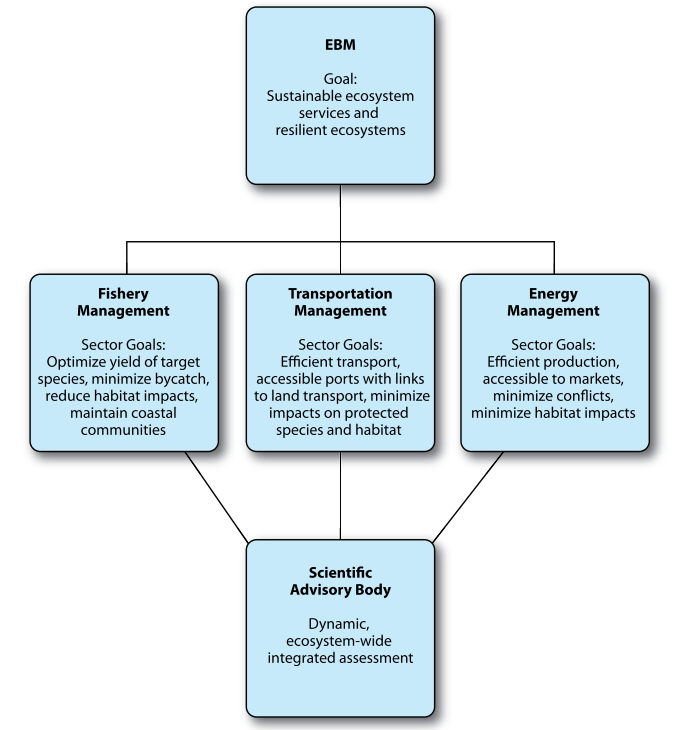
\includegraphics[width=90mm]{images/lubechenco-diagram.png}
  \caption {Framing ecosystem-based management goals, as in \cite{Lubchenco2010}; original from \citep{McLeod2009}}
  \label{fig:framing}
\end{figure}


% - shipping has big economic benefit, but costs are externalized

% - there are good actors in shipping who want to do the right thing, but don't have the tools to do it [cites, +Maersk lady]

% - only scientific community can do this

% - can only do msp by bringing stakeholders together

% - VGI methods provide good way of handling messy data as we try to move it toward 'reality'

% - coupling these approaches with real-time efforts has potential to shift dynamic.


% State what the data mean, link to question stated in the introduction

% - summarize results/findings
% - put results into context
% - explain implications
% - link to future work + highlight shortcomings

% XXX this paragraph imported from the original introduction, is it better here?
As noted by Goodchild, ``changing technology and economics are moving map production from a system of unified central production to a local patchwork, and the old radial system of dissemination is being replaced with a complex network''\citep{goodchild1999cartographic}. By using the quality assurance methods of record linkage and geographic validation, provides an approach to filter unreliable inputs of shipping data, and take advantage of the newly formed patchwork to broaden our understanding of ocean transportation. The near future will involve global, real-time, high resolution ship data \citep{JonesGoogle2012,carson2012satellite}, but we need methods which accommodate data curation and integration. By using quality assurange methods, I have shown that multiple data dimensions can be incorporated, and heterogenous errors can be rectified.

% This is a key appeal of volunteered information: some problems of uncertainty become tractable with sufficient observation volume, as we can evaluate the distribution directly instead of relying on sampling methods.

Recent calls for increased marine spatial planning at both the national and international level should be met with increased production of fundamental datasets required for effective planning. This work can help advancement of both marine spatial planning and ecosystem-based management, and to help organizations like the IMO provide more effective regulation of shipping, perhaps using insurance-based incentives to reflect environmental costs. The movement toward ubiquitous and real-time data provides an opportunity to greatly improve our management of ocean resources.

This work is a step toward understanging the global effects of shipping. True cost-path movements, which account for vessel preference and barriers, will give us a way of understanding the relative value of different areas within the ocean to the shipping industry. An abstract network model, which incorporates the detailed movement model developed, would allow us to interact with this complex data in a much simpler way, and potentially lead to breakthroughs in marine spatial planning at regional scales. More immediately, these results can feed into understanding the anthropogenic sources of sound in the ocean, and improve models of ship strikes, by providing detailed, holistic speed models for most of the oceans.
% The ship classifications should be derived rigorously, perhaps directly relying on observation data such as those presented here~\citep{adams2011constructing}.

% phantom ships phenomena



%\appendix{}
%\gdef\thesection{Appendix \Alph{section}}

\chapter{Movement Modeling}
\label{sec:movement-modeling-appendix}

% XXX copy and paste job, include details here.... tools used? DETAILED APPROACH.
Each vessel track was rasterized to both an 90 arcsecond grid (\textasciitilde{}5.5km at the equator) and an equal area grid in the Hobo Dyer projection (Figure \ref{fig:eu-cargo-density}). The latter case assures that the density function is computed on grid cells representing the same area for each cell, unlike the geographic grid where area varies by latitude. A vessel is counted only once for each cell it passes through, as the focus here on overall movement patterns, and this criteria helps de-emphasize vessels with limited movement. Each raster vessel track was combined using simple map algebra to produce density maps for both the AIS and VOS data, for each of our vessel classes. % XXX Oliver: A passing cargo ship is comparable to a ferry crisscrossing the same spot continuously every day?  Not that you should do this, but somebody might wonder.

Maps produced in ArcGIS and Quantum GIS.

gdal_rasterize did the rasterization step

gdal_add, custom python code combined the results

paralellized in Python.

% Bresenham's line algorithm used for rasterizing the tracks. Only counted a ship moving through a single cell once to get movement patterns v. dockage

% XXX built spatial indexes and reordered the data on disk to match for performance.


\chapter{Record Linkage}
\label{sec:record-linkage-appendix}

The Jaro-Winkler formula is defined in two steps. First, The Jaro distance, $d_j $, is defined as:

% good code-based illustration at: http://www.gettingcirrius.com/2011/01/calculating-similarity-part-2-jaccard.html

\begin{equation}
  d_j = \left\{
  \begin{array}{l l}
    0 & \text{if }m = 0 \\ 
    \frac{1}{3}\left(\frac{m}{|s_1|} + \frac{m}{|s_2|} + \frac{m-t}{m}\right) & \text{otherwise} \end{array} \right.
\end{equation}

Where:

m = number of matching patterns
t = number of transposed characters
|s1| = length of first string
|s2| = length of second string

Two characters are considered matching when they are no further apart than:
\begin{equation}
  \left\lfloor\frac{\max(|s_1|,|s_2|)}{2}\right\rfloor-1
\end{equation}

The second component, added by Winkler, preferentially weights strings which match from the beginning, set by the prefix length $ l $.  Thus, the Jaro-Winkler distance is defined:

\begin{equation}
  d_w = d_j + (\ell p (1 - d_j))
\end{equation}

Where $ p $ is a constant scaling factor to adjust for the strength of common prefixes. In its usage here, $ p = 0.1 $ and $ l = 4 $.



\chapter{Tables}

\begin{table}[htbp]
  \begin{tabular}{lr}
    Attribute & Accuracy \\
    \hline
    Location (fixed from GPS signal) & $\simeq$10 meter accuracy) \\
    Timestamp (on broadcast) & $\simeq$100 ms \textit{radio transmission \& processing latency}\\
    Name \\
    Call Sign \\
    Maritime Mobile Service Identity (MMSI) \\
    Heading \\
    Speed \\
    Destination & \textit{rarely valid}
  \end{tabular}
  \caption[AIS broadcast attributes]{AIS broadcast attributes. Update frequency depends on ship speed, but varies between a minimum of a record every 2 seconds for quickly moving vessels, to once per 3 minutes for moored vessels. Additional attributes are available, but infrequently used.}
  \label{table:ais-broadcast-attributes}
\end{table}

% had this as a list, also some hackery with unnesting class data:
% select distinct(trim(both from unnest(class))), count(*) from clean.ships where validation_class = 'tanker' and validation_score > 0 and obs_count > 0 GROUP BY class ORDER BY btrim DESC;ships=# select distinct(trim(both from unnest(class))), count(*) from clean.ships where validation_class = 'tanker' and validation_score > 0 and obs_count > 0 GROUP BY class ORDER BY btrim DESC;

\begin{longtable}{l|l|l}
\hline \multicolumn{1}{|c|}{\textbf{Type}} & \multicolumn{1}{c|}{\textbf{Sub-type}} & \multicolumn{1}{c|}{\textbf{Vessels}} \\ \hline 
\endfirsthead

%\multicolumn{3}{c}%
%{{\bfseries \tablename\ \thetable{} -- continued from previous page}} \\
\hline \multicolumn{1}{|c|}{\textbf{Type}} &
\multicolumn{1}{c|}{\textbf{Sub-type}} &
\multicolumn{1}{c|}{\textbf{Vessels}} \\ \hline 
\endhead

%\hline \multicolumn{3}{|r|}{{Continued on next page}} \\ \hline
\endfoot
    cargo & cargo ship & 30355 \\
          & merchant & 2919 \\
          & bulk carrier & 1338 \\
          & container ship & 669 \\
          & general cargo & 608 \\
          & vehicle carrier & 56 \\
    tanker & tankship & 10460 \\
           & tanker   & 8731 \\
           & oil tanker & 1312 \\
           & liquefied gas carrier & 112 \\
           & chemical carrier & 39 \\
    other & merchant & 17460 \\
          & other ship & 9421 \\
          & unspecified & 4580 \\
          & motor boat & 4231 \\
          & inland waterways & 3825 \\
          & sloop & 2799 \\
          & reserved for future use & 2164 \\
          & all other activities & 1345 \\
          & reserved for regional use & 712 \\
  support & pusher/tug & 4392 \\
          & tug & 7885 \\
          & towing vessel & 2747 \\
          & supply vessel & 1501 \\
          & service vessels & 1388 \\
          & trawler & 1056 \\
          & dredger & 995 \\
          & vessel engaged in dredging or underwater operation & 776 \\
          & pilot vessel & 685 \\
  pleasure & pleasure/leisure & 22013 \\
           & pleasure & 14573 \\
           & pleasure craft & 7290 \\
           & sailing vessel & 5527 \\
           & yacht & 8214 \\
  fishing & fishing vessel & 11110 \\
          & fishing boat & 8454 \\
          & fishing industry & 5767 \\
          & fishing & 3213 \\
  passenger & passenger ship & 6478 \\
            & ferry & 704 \\
  high-speed & high-speed craft & 658 \\
             & high speed craft & 520 \\
  authority & sar-vessel & 699 \\
            & search and rescue vessel & 609 \\
            & rescue vessel & 102 \\
  \caption[Detailed ship classes]{Detailed ship class breakdown. Classes come from observationsgT}
  \label{table:ship-class-breakdown}
\end{longtable}

%\newpage
%\chapter{Source Code}
%\label{sec:source-code}

% include SOME python code here -- our AIS parser, what else?
% steps: download AIS
% parse ais
% insert AIS into DB, formalize
% download & parse ship databases

%All code used to generate the project is available at https://github.com/scw/ais-kml-parser. The full code is omitted from this document, due to length restrictions.

%\texttt{aiskml.py}:
%\inputminted[linenos,
%             numbersep=5pt,
%             frame=lines,
%             framesep=2mm]{r}{../code/kml/aiskml.py}

%\texttt{parsekml.py}:
%\inputminted[linenos,
%             numbersep=5pt,
%             frame=lines,
%             framesep=2mm]{r}{../code/kml/parsekml.py}

\chapter{Figures}
\label{sec:figures}

\begin{figure}[htbp]
  \centering
  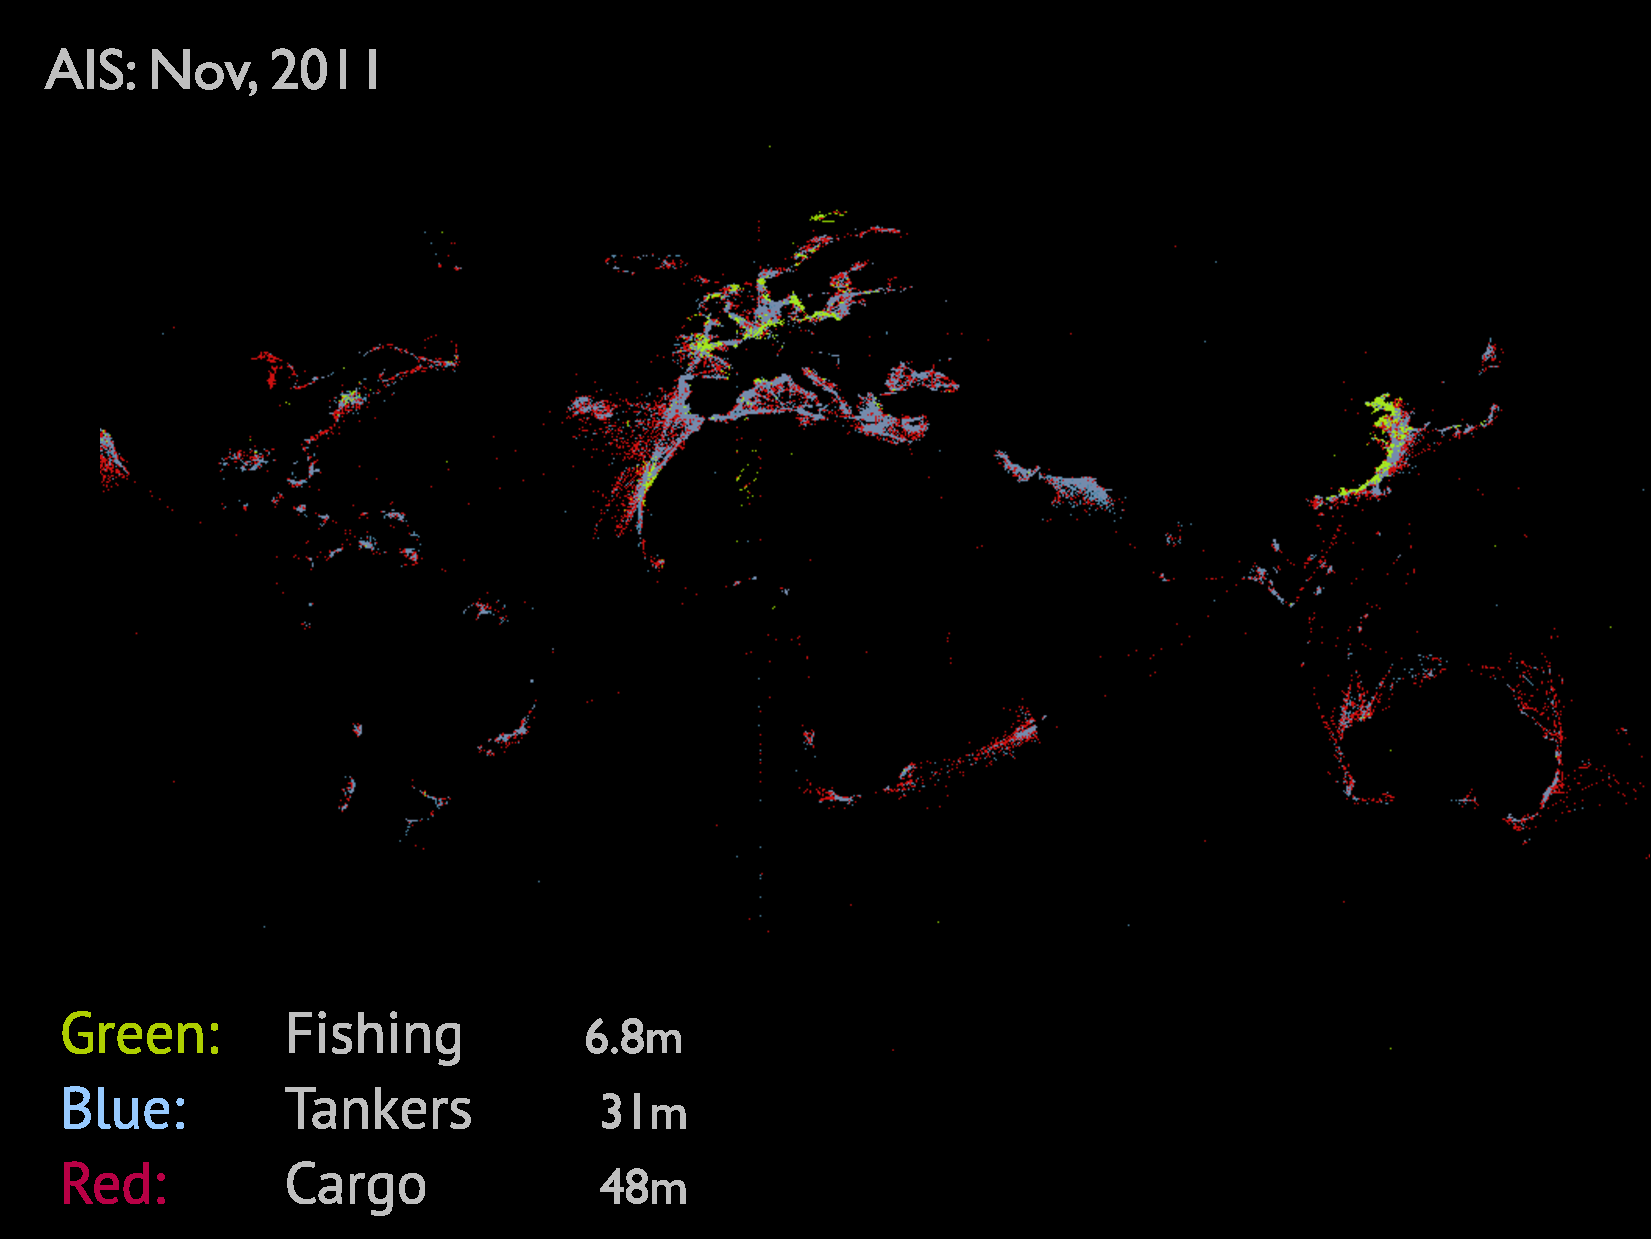
\includegraphics[width=160mm]{figures/ais-nov-2011.pdf}
  \caption[AIS observations, November 2011]{Raw AIS observations, November 2011. Note the observations located in the Hoggar Mountains in Algeria.}
  \label{fig:ais-obs-nov-2011}
\end{figure}

% show our image of invalid 'on land' ships in the harbor of long beach?
\begin{figure}[htbp]
  \centering
  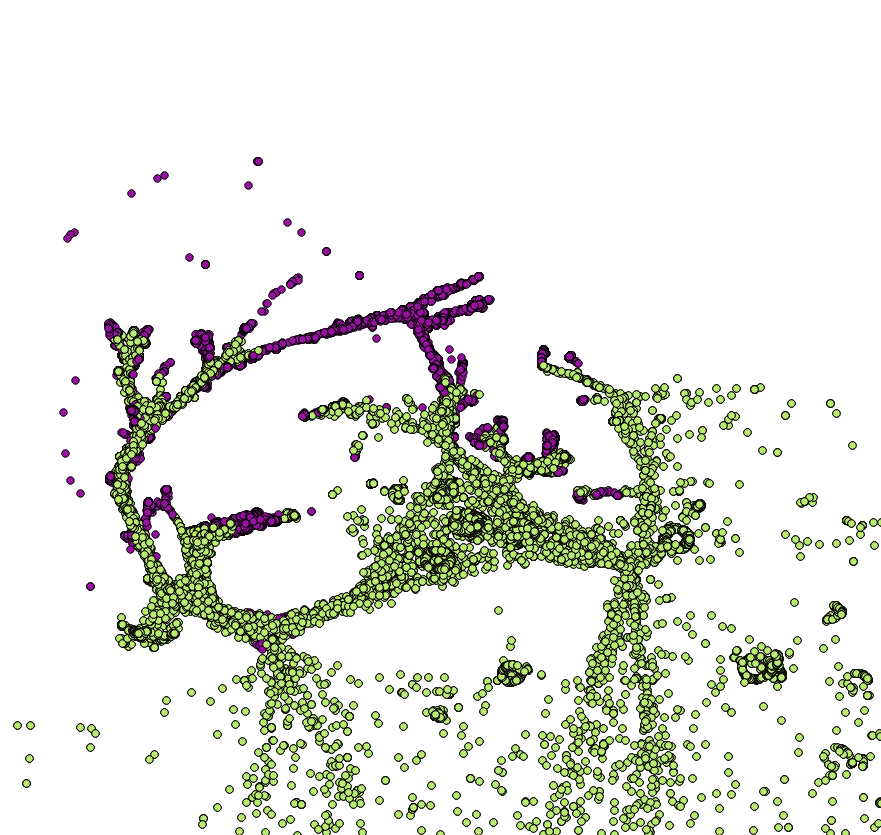
\includegraphics[width=140mm]{figures/example-long-beach-harbor-validation.png}
  \caption[Long beach harbor, validation example]{Long Beach Harbor, California. Points shown here in purple are 'on land', but most of these on-land observations are actually parts of the harbor.} % XXX Oliver: a little context here?
  \label{fig:longbeach-validation}
\end{figure}


\begin{figure}[htbp]
  \centering
  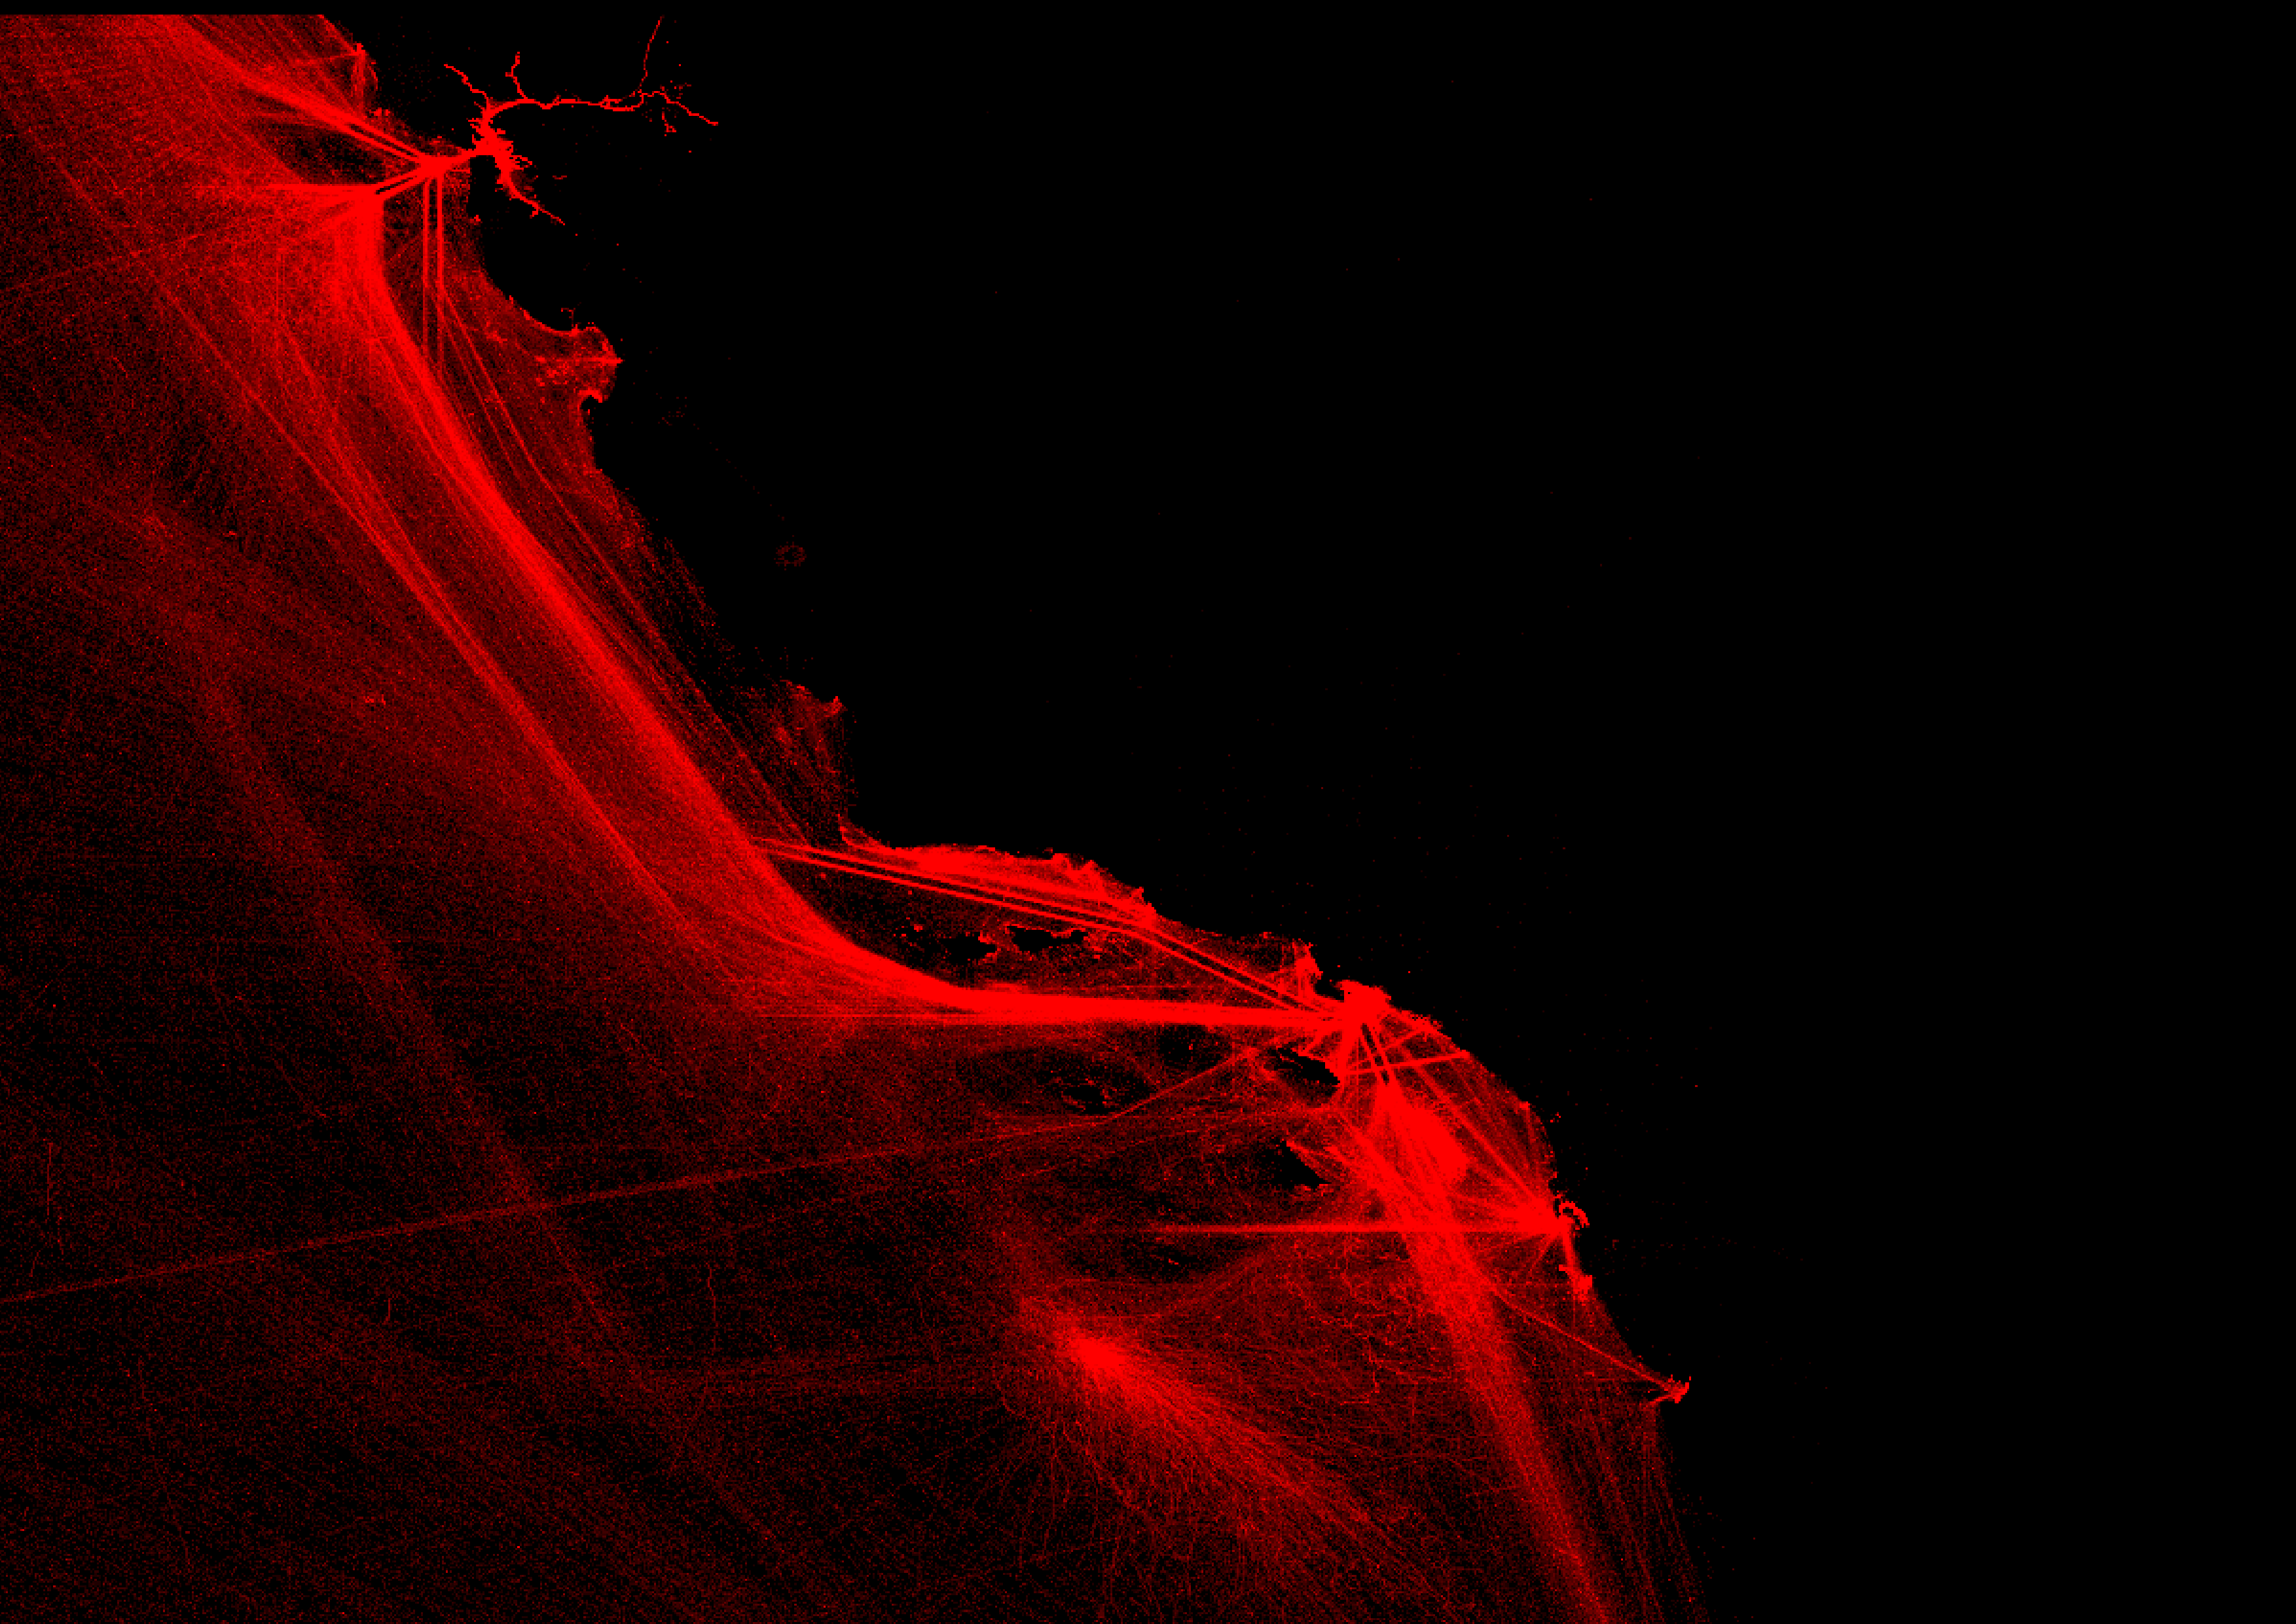
\includegraphics[width=140mm]{figures/cargo_density.png}
  \caption[AIS Observations, Southern California Bight]{AIS observations, Southern California Bight. Nov 2010--Dec 2011. Note the ballast water exchange point lower left.}
  \label{fig:cal-cargo}
\end{figure}

\begin{figure}[htbp]
  \centering
  \includegraphics[width=160mm]{figures/ais-and-ports-cea.pdf}
  \caption[AIS coverage]{Approximate AIS coverage (green), global ports (red).}
  \label{fig:ais-coverage}
\end{figure}

\begin{figure}[htbp]
  \centering
  \includegraphics[width=160mm]{figures/cia-lanes-small-cropped.png}
  \caption[CIA World Shipping Lanes]{"World Shipping Lanes" map produced by the Central Intelligence Agency, 1973.}
  \label{fig:cia-shipping-map}
\end{figure}




\bibliography{refs/thesis,refs/links,refs/vgi,refs/prospectus,refs/standards,refs/software}
%\bibliographystyle{plainnat}
\bibliographystyle{jss}
\end{document}
